\documentclass{beamer}

\usepackage[utf8]{inputenc}
\usepackage[french]{babel}
\usepackage{graphicx}

\graphicspath{ {img/} }

%\definecolor{fondtitre}{RGB}{0,113,178}
\definecolor{coultitre}{RGB}{0,113,178}
\setbeamercolor{structure}{fg=coultitre}


\title{Mail}

% A subtitle is optional and this may be deleted
\subtitle{Définition / Application / Protocoles}

\author{C.~Desgenetez \and J.~Guillen}
% - Give the names in the same order as the appear in the paper.
% - Use the \inst{?} command only if the authors have different
%   affiliation.

\institute[Faculté des sciences de Montpellier] % (optional, but mostly needed)

% \subject{Theoretical Computer Science}


\AtBeginSubsection[]
{
  \begin{frame}<beamer>{Sommaire}
    \tableofcontents[currentsection,currentsubsection]
  \end{frame}
}

% Let's get started
\begin{document}

\begin{frame}
  \titlepage
\end{frame}
\begin{frame}
    \begin{itemize}
        \item{
            204 millions d’e-mails envoyés par minute dans le monde
        }
        \item{
            25\% des courriers électroniques sont lus par le destinataire dans l’heure qui suit leur envoi
        }
        \item{
             75\% des courriers traités par les serveurs de messagerie sont des "spams" 
        }
        \item{
             564 milliards d’emails par jour ("spams" inclus)
        }
        \item{
              2 heures par jour. C’est le temps que consacrent en moyenne les cadres \`à la lecture de leurs e-mails, selon l’Observatoire de la responsabilité sociétale des entreprises.
        }
    \end{itemize}
\end{frame}
\begin{frame}{Sommaire}
  \tableofcontents
  % You might wish to add the option [pausesections]
\end{frame}

% Section and subsections will appear in the presentation overview
% and table of contents.
\section{Le mail}

    \subsection{1.Histoire et étymologie}
    
\begin{frame}{Le mail}{Histoire et étymologie}
    \begin{block}{Histoire}
    \begin{itemize}
        \item{
            Inventé en 1965 sur CTSS (Compatible time-sharing system) du MIT
        }
        \item<2->{
            Première utilisation par Ray Tomlinson en 1971.\\
            Sur le réseaux Arpanet avec comme contenu "QWERTY".
        }
        \item<3->{
            Caractère inutilisé "@"
        }
    \end{itemize}
    \end{block}
    \begin{block}{\'Etymologie}
    \begin{itemize}
        \item<4-> {
         Mail vient de malleus qui veut dire marteau en latin.
         Notamment utilisé dans le jeu de mail.
        }
        \item<5-> {
        Mail prononcé "maille" est une allée avec des arbres, à la base réservée au jeu de mail.    
        }

    \end{itemize}
    \end{block}
\end{frame}

\subsection{2.Principe et définition}
\begin{frame}{Le mail}{Définition}
    \begin{block}{Définition}
        \begin{itemize}
            \item<1-> {
                Mail : Lettre informatique pouvant contenir différents documents sous divers formats    (pdf, image, musique).
                    }
             \item<2-> {
                Mail est aussi une commande Unix \newline
                mail -s "Sujet du mail" adresse1@exemple1.com
                }
            \item<3-> {
                Client de messagerie : Application permettant l'écriture et l'envoi de mails.\newline
                ex: Gmail}
            \item<4-> {
                Client local.\newline
                ex: Mozilla Thunderbird...}
            \item<5->{
                Client web.
                ex: Yahoo Mail...
                }
      \end{itemize}
    \end{block}
\end{frame}
\begin{frame}{Le mail}{Principe}
    \begin{figure}[h]
        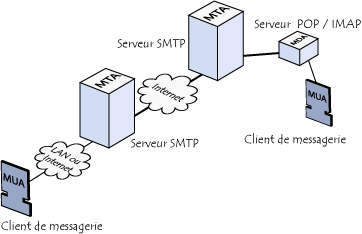
\includegraphics[width=0.80\textwidth, ]{mailT} 
        \caption{} 
        \label{fig:mesh2}
    \end{figure}
\end{frame}
\begin{frame}{Le mail}{Principe}
    \begin{figure}[h]
        
\includegraphics[width=0.90\textwidth, ]{shemaM} 
        \caption{} 
        \label{fig:mesh1}
    \end{figure}
    \begin{itemize}
        \item {
            MUA (Mail User Agent) : Client de messagerie.
            }

  % or you can use the \uncover command to reveal general
  % content (not just \items):
        \item<2-> {
            MTA (Mail Transport Agent) : Serveur chargé du transport du message. \uncover<3-> {Protocoles SMTP.}  }
   
        \item<4-> {
            MDA (Mail Delivery Agent) : Serveur de stockage.\uncover<5->{ Protocoles POP3 ou IMAP.}
            }
  \end{itemize}
\end{frame}




\subsection{3.Législation}
\begin{frame}{Le mail}{Législation}
    \begin{itemize}
        \item<1->{      
            Mode de communication valable professionnellement, si les deux parties fournissent une adresse. \nextline            
            Engagement à ce que l'adresse soit valide et consultée régulièrement.
        }
        \item<2->{
            Un mail vaut autant qu'un écrit papier en tant que preuve.\\
            Il est aussi valable pour conclure un contrat selon trois règles:
            \begin{itemize}
                \item 1. La signature doit identifier son auteur.
                \item 2. Le procédé doit garantir le lien entre la signature et le contrat.
                \item 3. Le contrat doit être intègre.
            \end{itemize}
        }  
        \item<3->{
            L'adresse professionnelle peut être utilisée à but personnel.
        }
    \end{itemize}
\end{frame}


\section{Les applications}

    \subsection{1.Définition d'une application}
        \begin{frame}{Les applications}{Définition}
            \begin{itemize}
                \item {
                    Programme directement utilisé par l'utilisateur.
                }
                \item<2-> {
                    Utilise les services du système d'exploitation pour utiliser les ressources matérielles.
                }
                \item<3->{
                    Exemple: éditeur de texte, navigateur web, jeux vidéo ...
                }
            \end{itemize}
        
        \end{frame}
    \subsection{2.Application mail locale}
        \begin{frame}
        \begin{block}{Client de messagerie}
            \begin{itemize}
                \item {
                    Installé sur la machine du client.
                }
                \item {
                    Stocke les messages de façon locale.
                }
                \item{
                    Regroupent différentes adresses mails.
                }
                \item{
                    Contrôle des données sauvegardées
                }
            \end{itemize}
            \end{block}
        \end{frame}
    \subsection{3.Application mail web}
        \begin{frame}
        \begin{block}{Webmail}
            \begin{itemize}
                \item {
                Webmail : Client de messagerie sur serveur web.\\
                }
                \item {
                    Installée sur un serveur et nécessite un naviguateur web.
                }            
                \item {
                Préconfiguré.
                }
                \item {
                Problèmes de sécurité de l'information.
                }
                \begin{itemize}
                    \item Propriétaire : Yahoo mail, gmail, Outlook...
                    \item Open source : roundcube...
                \end{itemize}
            \end{itemize}
            \end{block}
        \end{frame}
% \section{Les protocoles}

%     \subsection{1.Définition d'un protocole}
%     \subsection{2.Protocole serveur}
%     \subsection{3.Protocole client}


% Note a moi même :
% http://jetel.free.fr/inf_rsx.htm
% https://fr.wikipedia.org/wiki/Couche_application
% https://fr.wikipedia.org/wiki/Mod%C3%A8le_OSI
% https://fr.wikipedia.org/wiki/Liaison_point_%C3%A0_point


\section{Les protocoles}
    \subsection{1.Définitions}
    
\begin{frame}{Les protocoles}{Définition d'un protocole}
  \begin{block}{Définitions}
  \begin{itemize}
    \item<1->{
    Protocole:\\
    Ensemble de règles définissant le mode de communication entre deux ordinateurs.
    }
  \item<2->{
    Encapsulation:\\
    Procédé consistant à inclure les données d'un protocole dans un autre protocole.
    }
%   \item<3->{
%     Modèle OSI:\\
%     \textbf{O}pen \textbf{S}ystems \textbf{I}nterconnection
%     }
  \end{itemize}
  \end{block}
\end{frame}


% \begin{frame}{Les protocoles}{Modèle OSI}
% \begin{example}
%     \begin{figure}[H]
%     \centering
%     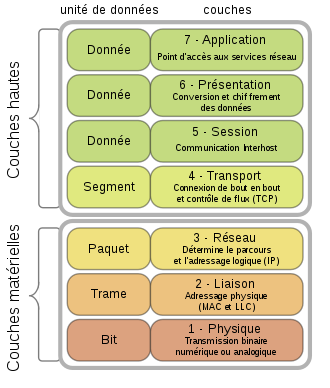
\includegraphics[width=0.4\textwidth]{OSI_Model_v1}
%      \caption{Modèle OSI}
%      \label{fig:mode_osi}
%     \end{figure}
% \end{example}
% \end{frame}

\subsection{2.Protocole serveur}
\begin{frame}{Les protocoles}{Protocole serveur}
  \begin{block}{SMTP}
  \begin{itemize}
    \item<1->{
    \textbf{S}imple \textbf{M}ail \textbf{T}ransfer \textbf{P}rotocol\\
    (Protocole Simple de Transfert de Courrier)
    }
  \item<2->{
    D'un serveur à un autre. 
    }
   \item<3->{
    TCP/IP
    }
    \item<4->{
    Commandes textuelles.
    }
    \item<5->{
    Ne permet pas de récupérer à distance des courriels arrivés dans une boîte aux lettres sur un serveur.
    }
  \end{itemize}
  \end{block}
\end{frame}

\begin{frame}{Les protocoles}{Protocole serveur}
\begin{example}
    \begin{figure}[H]
    \centering
    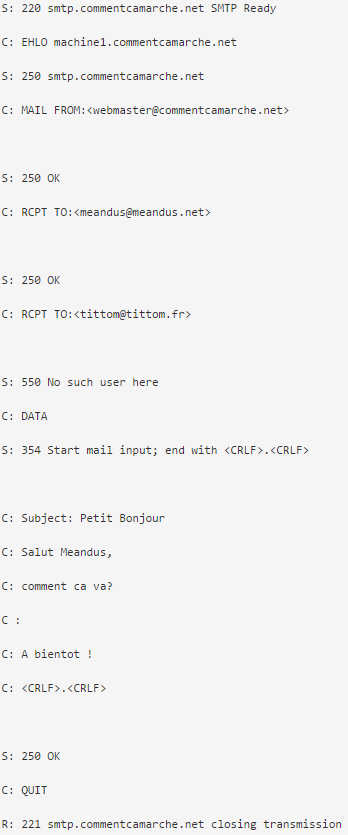
\includegraphics[width=0.6\textwidth]{message_smtp}
     \caption{Exemple de commandes textuelles SMTP}
     \label{fig:commande_text_SMTP}
    \end{figure}
\end{example}
\end{frame}


\begin{frame}{Les protocoles}{Protocole serveur}
  \begin{block}{SMTP}
  \begin{itemize}
    \item<1->{
    Port par défaut \\
    \begin{itemize}
        \item 25 (sans chiffrement) 
        \item 587 (avec chiffrement)
        \item 465 (SSL)
        \item 587 (TLS)
    \end{itemize}
    }
  \end{itemize}
  \end{block}
\end{frame}

\begin{frame}{Les protocoles}{Protocole serveur}
  \begin{block}{SMTP}
  \begin{itemize}
    \item<1->{
     2006, l'AFA recommande aux FAI de bloquer les paquets TCP/IP sortant à destination du port 25.
    }
    \item<2->{
    50\% et 80\% du spam était généré par des ordinateurs infectés
    }
    \item<3->{
    SMTP authentifié (port 587)
    }
    \item<4->{
    Port 25 sert uniquement aux serveurs SMTP entre eux.
    }
  \end{itemize}
  \end{block}
\end{frame}

\subsection{2.Protocole client}
\begin{frame}{Les protocoles}{Protocole client}
  \begin{block}{POP3 et IMAP}
  \begin{itemize}
    \item<1->{
    POP3:\\
    \textbf{P}ost \textbf{O}ffice \textbf{P}rotocol Version 3
    } 
    \item<2->{
    IMAP:\\
    \textbf{I}nternet \textbf{M}essage \textbf{A}ccess \textbf{P}rotocol
    }
  \item<3->{
    D'un client à un autre. 
    }
   \item<4->{
    TCP/IP
    }
    \item<5->{
    Commandes textuelles.
    }
  \end{itemize}
  \end{block}
\end{frame}

\begin{frame}{Les protocoles}{Protocole client}
\begin{example}
    \begin{figure}[H]
    \centering
    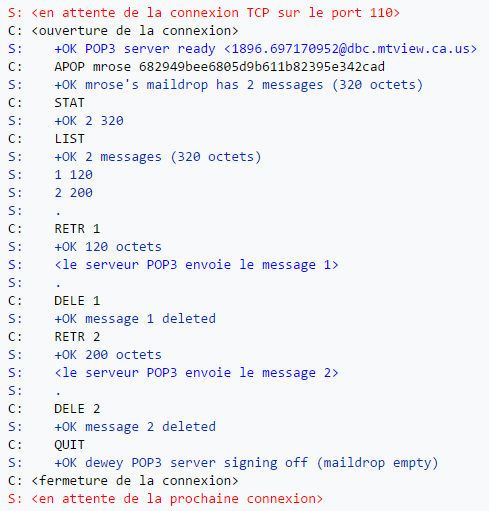
\includegraphics[width=0.6\textwidth]{pop_message}
     \caption{Exemple de commandes textuelles POP}
     \label{fig:commande_text_POP}
    \end{figure}
\end{example}
\end{frame}

\begin{frame}{Les protocoles}{Protocole client}
  \begin{block}{POP}
  \begin{itemize}
  \item<1->{
  Transfère du serveur au client puis efface du serveur.
  }
    \item<2->{
    Port par défaut \\
    \begin{itemize}
        \item 109 POP2
        \item 110 POP3
        \item 995 POP3 (TLS)
    \end{itemize}
    }
    \item<3->{
     Serveurs libre: OpenSMTPD, Postfix, qmail...
    }
  \end{itemize}
  \end{block}
\end{frame}

\begin{frame}{Les protocoles}{Protocole client}
  \begin{block}{SMTP}
  \begin{itemize}
    \item<1->{
      Synchronisation des messages et des dossiers
      }
    \item<2->{
    Port par défaut \\
    \begin{itemize}
        \item IMAP2 et IMAP4: 143
        \item IMAP3: 220
        \item IMAPS (SSL): 993
    \end{itemize}
    }
    \item<3->{
     Serveurs libre: Cyrus, Dovecot...
    }
  \end{itemize}
  \end{block}
\end{frame}

\begin{frame}{Les protocoles}{Protocole client}
    \begin{figure}[H]
    \centering
    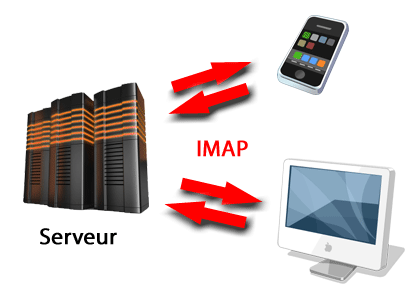
\includegraphics[width=0.6\textwidth]{imap_schem}
     \caption{IMAP}
     \label{fig:imap}
    \end{figure}
\end{frame}


\begin{frame}{Les protocoles}{Protocole client}
  \begin{block}{Serveur SMTP / IMAP,POP3}
  \begin{itemize}
    \item<1->{
    Libre : BlueMind, Zimbra...
    }
    \item<2->{
     Propriétaires : Mail Server (Apple), Microsoft Exchange Server...
    }
  \end{itemize}
  \end{block}
\end{frame}



\begin{frame}
\begin{block}{Sources}
\begin{itemize}
    \item http://www.commentcamarche.net
   
    \item Wikipedia
    
    \item https://expertsecuritedigitale.blogspot.fr/2017/04/la-securiteappliquee-aux-courriers.html
    
    \item http://jetel.free.fr/inf\_rsx.htm
\end{itemize}
\end{block}
\end{frame}

\end{document}


